\documentclass[anon,12pt]{colt2021} % Anonymized submission
%\documentclass[final]{colt2020} % Anonymized submission
% \renewcommand{\includegraphics}[1][1]{}

% \documentclass{colt2020} % Include author names

% The following packages will be automatically loaded:
% amsmath, amssymb, natbib, graphicx, url, algorithm2e


\usepackage{times}

\usepackage{lmodern}
\usepackage{hyperref}       % hyperlinks  %[implicit=false, bookmarks=false]
\usepackage{booktabs}       % professional-quality tables
\usepackage{amsfonts}       % blackboard math symbols
\usepackage{nicefrac}       % compact symbols for 1/2, etc.
\usepackage{microtype}      % microtypography

\PassOptionsToPackage{numbers, sort, compress}{natbib}

\usepackage{mathtools, verbatim}
%\usepackage[thmmarks, thref, amsthm]{ntheorem}
\usepackage{color}
\definecolor{darkblue}{rgb}{0.0,0.0,0.2}
\definecolor{darkgreen}{rgb}{0.0,0.3,0.0}
\hypersetup{colorlinks,breaklinks,
	linkcolor=darkblue,urlcolor=darkblue,
	anchorcolor=darkblue,citecolor=darkblue}
\usepackage{wrapfig}
\usepackage[small]{caption}
% NOTE: had to comment out "todo" in colt2021.cls
\usepackage[colorinlistoftodos,textsize=tiny]{todonotes} % need xargs for below
%\usepackage{accents}
\usepackage{bbm}
\usepackage{xspace}
\usetikzlibrary{arrows}
\usetikzlibrary{shapes}

\makeatletter
\let\Ginclude@graphics\@org@Ginclude@graphics 
\makeatother

%\usetikzlibrary{calc}
\newcommand{\Comments}{1}
\newcommand{\mynote}[2]{\ifnum\Comments=1\textcolor{#1}{#2}\fi}
\newcommand{\mytodo}[2]{\ifnum\Comments=1%
	\todo[linecolor=#1!80!black,backgroundcolor=#1,bordercolor=#1!80!black]{#2}\fi}
\newcommand{\raf}[1]{\mynote{darkgreen}{[RF: #1]}}
\newcommand{\raft}[1]{\mytodo{green!20!white}{RF: #1}}
\newcommand{\jessie}[1]{\mynote{teal}{[JF: #1]}}
\newcommand{\jessiet}[1]{\mytodo{teal!20!white}{JF: #1}}
\newcommand{\bo}[1]{\mynote{blue}{[Bo: #1]}}
\newcommand{\botodo}[1]{\mytodo{blue!20!white}{[Bo: #1]}}
\newcommand{\btw}[1]{}%\mytodo{orange!80!white}{BTW: #1}}
\newcommand{\discuss}[1]{\mynote{cyan!20!white}{#1}}
\ifnum\Comments=1               % fix margins for todonotes
\setlength{\marginparwidth}{1in}
\fi

\newcommand{\reals}{\mathbb{R}}
\newcommand{\posreals}{\reals_{>0}}%{\reals_{++}}
\newcommand{\simplex}{\Delta_\Y}
\newcommand{\relint}[1]{\mathrm{relint}(#1)}
\newcommand{\interior}{\mathrm{int}\,}
\newcommand{\prop}[2][\mathcal{P}]{\mathrm{prop}_{#1}[#2]}
\newcommand{\elic}{\mathrm{elic}}
\newcommand{\eliccvx}{\mathrm{elic}_\mathrm{cvx}}
\newcommand{\conscvx}{\mathrm{cons}_\mathrm{cvx}}
\newcommand{\elicpoly}{\mathrm{elic}_\mathrm{pcvx}}
\newcommand{\elicembed}{\mathrm{elic}_\mathrm{embed}}
\newcommand{\ccdim}{\mathtt{cc\,dim}}
\newcommand{\rank}{\mathrm{rank}}
\newcommand{\proj}{\mathrm{proj}}
\newcommand{\supp}{\mathrm{supp}}
\newcommand{\spn}{\mathrm{span}}
\newcommand{\embed}{\mathtt{embed}}

\newcommand{\range}{\mathrm{range}\,}
\newcommand{\zeros}[1]{\mathrm{ker}_\P\,#1}
\newcommand{\codim}{\mathrm{codim}}
\newcommand{\Pcodim}{\mathcal{P}\!\text{-}\mathrm{codim}}
\newcommand{\Pcodimension}{$\mathcal{P}$-codimension\,}

\newcommand{\propdis}{\mu}
\newcommand{\affhull}{\mathrm{affhull}}
\newcommand{\epi}{\mathrm{epi}}
\newcommand{\cl}{\mathbf{cl}}
%\newcommand{\span}{\mathrm{span}}

\newcommand{\A}{\mathcal{A}}
\newcommand{\C}{\mathcal{C}}
\newcommand{\D}{\mathcal{D}}
\newcommand{\E}{\mathbb{E}}
\newcommand{\F}{\mathcal{F}}
\renewcommand{\H}{\mathcal{H}}
\renewcommand{\L}{\mathcal{L}}
\newcommand{\Lcvx}{\mathcal{L}^{\mathrm{cvx}}}
\newcommand{\I}{\mathcal{I}}
\newcommand{\N}{\mathcal{N}}
\newcommand{\R}{\mathcal{R}}
\renewcommand{\P}{\mathcal{P}}
\newcommand{\Sc}{\mathcal{S}}  % jessie, feel free to redef, just not \S :-)
\newcommand{\Scr}{\mathcal{S}}  % using this for the span of F_p - not sure if we want this to be parallel to the feasible subspace notation
\newcommand{\U}{\mathcal{U}}
\newcommand{\V}{\mathcal{V}}
\newcommand{\X}{\mathcal{X}}
\newcommand{\Y}{\mathcal{Y}}


\newcommand{\ellbar}{\underline{\ell}}
\newcommand{\lbar}{\underline{L}} % couldn't do L* while proofreading...
\newcommand{\iden}{\mathrm{iden}}
\newcommand{\im}{\mathrm{im}}
\newcommand{\Var}{\mathrm{Var}}
\newcommand{\CVaR}{\mathrm{CVaR}}

\newcommand{\exploss}[3]{\E_{#3} #1(#2,Y)}
\newcommand{\risk}[1]{\underline{#1}}
\newcommand{\Ind}[1]{\mathbf{I}\{{#1}\}}
\newcommand{\inprod}[2]{\langle #1, #2 \rangle}
\newcommand{\toto}{\rightrightarrows}
\newcommand{\ones}{\mathbbm{1}}

%\newtheorem{theorem}{Theorem}
%\newtheorem{lemma}{Lemma}
%\newtheorem{proposition}{Proposition}
%\newtheorem{corollary}{Corollary}
%\newtheorem{conjecture}{Conjecture}
%\newtheorem{definition}{Definition}
\newtheorem{assumption}{Assumption}
\newtheorem{condition}{Condition}
\newtheorem{openq}{Open Question}
%\newtheorem{remark}{Remark}


\DeclareMathOperator*{\argmax}{arg\,max}
\DeclareMathOperator*{\argmin}{arg\,min}
\DeclareMathOperator*{\arginf}{arg\,inf}
\DeclareMathOperator*{\sgn}{sgn}

\usepackage{thmtools, thm-restate}
%\declaretheorem{corollary}



% The \author macro works with any number of authors. There are two commands
% used to separate the names and addresses of multiple authors: \And and \AND.
%
% Using \And between authors leaves it to LaTeX to determine where to break the
% lines. Using \AND forces a line break at that point. So, if LaTeX puts 3 of 4
% authors names on the first line, and the last on the second line, try using
% \AND instead of \And before the third author name.

%Indirect elicitation as a necessary condition for consistent surrogate losses
\title{Lower bounds on convex consistent surrogates for abstain loss}

% Three or more authors with the same address:
\coltauthor{\Name{Jessie Finocchiaro} \Email{jessica.finocchiaro@colorado.edu}\\
	\Name{Rafael Frongillo} \Email{raf@colorado.edu}\\
	\Name{Bo Waggoner} \Email{bwag@colorado.edu}\\
	\addr CU Boulder}



\begin{document}
\maketitle

\begin{abstract}
We study the problem of constructing consistent surrogates that abstain from classification when given data points with low confidence over the likelihood of the outcomes.
Particularly, we review lower bounds on the dimensionality required to learn construct a \emph{consistent, convex} loss function that abstains in low-confidence settings.
\end{abstract}

\section{Introduction}
In \emph{empirical risk minimization} (ERM), supervised machine learning algorithms learn to make predictions about future inputs by learning a hypothesis function that minimizes a given loss function over a labeled training dataset.
The loss function used often naturally corresponds to the question at hand; 0-1 loss is used for multiclass classification, squared loss is used to predict the expected value, and pinball loss is used to learn quantiles.
The task at hand corresponds to the loss function optimized; often, these losses can be discrete, and therefore $NP$-hard to optimize, motivating the study of surrogate losses that are easier to optimize.
In particular, we restrict to the study of \emph{consistent, convex} surrogate losses for the \emph{abstain problem}.
In the abstain problem, we want our machine learning algorithm to abstain and defer classification to a human when the algorithm has low confidence over the labels on a given input.
We present and review some of the previous consistent surrogates for the abstain problem, and discuss the minimum dimension of a convex loss that learns this task in a statistically consistent manner.

We consider surrogates $L:\reals^d \times \Y \to \reals_+$ for a given discrete loss corresponding to the task of interest.
Here, we call $d$ the dimension of the surrogate, and we aim to understand how to construct surrogates of low dimension (in the number of outcomes), as this contributes to lowering the complexity of the optimization problem as a whole.
However, when we require surrogate to be consistent, this imposes a natural tension with finding one that is efficient in the prediction dimension $d$, as increasing the dimensional allows for more degrees of freedom to link surrogate predictions back to their discrete analogous predictions.

%\jessie{Discuss consistency and how elicitation is a necessary condition}
%\subsection{Property elicitation}
%\jessie{Try to write without properties}
%Simply put, \emph{properties} are functions mapping distributions over outcomes to reports.
%\begin{definition}[Property, elicits, level set]
%		A \emph{property} is a (possibly set-valued) function $\Gamma : \simplex \toto \R$ mapping distributions to reports.
%	A loss $L : \R \times \Y \to \reals_+$ \emph{elicits} the property $\Gamma$ if,
%	\begin{equation}
%	\forall p \in \simplex, \;\; \Gamma(p) = \arginf_{u \in \R} \E_{Y \sim p}L(u, Y)
%	\end{equation}
%	Moreover, we call a \emph{level set} $\Gamma_r := \{p \in \simplex : r \in \Gamma(p)\}$ to be the set of distributions for which reporting $u$ minimizes the expected loss of the loss eliciting $\Gamma$.
%\end{definition}

\section{The abstain loss}
In this work, we particularly focus on the \emph{abstain loss}.
Given a constant $\alpha \in (0,1)$, the abstain loss is a variation of cost-sensitive classification which allows for a constant punishment $\alpha$ for ``abstaining,'' represented here by the report $\bot$.

\begin{equation}
\ell^\alpha(r,y) = \begin{cases}
0 & r = y \\
\alpha & r = \bot\\
1 & r \not \in \{y, \bot\}
\end{cases}\tag*{Abstain loss}
\end{equation} 

In order to obtain ERM bounds on learning the abstain problem, we want to optimize a consistent surrogate $L^\alpha$, roughly meaning there is a link $\psi$ such that approaching the $L^\alpha$-optimal hypothesis implies applying the link $\psi$ leads to approaching the $\ell^\alpha$-optimal hypothesis.
\citet{bartlett2006convexity,ramaswamy2016convex} \jessie{add full list here} show that consistency and \emph{calibration} are equivalent notions.

%Ideally, one wants to learn a hypothesis function $h$ to minimize this loss in expectation for any distribution $D$ over $\X \times \Y$.
%However, if the hypothesis class $\H$ is sufficiently rich to contain the Bayes optimal classifier, we can focus on what the optimal classifier $h^*(x)$ should predict in order to minimize $\E_{Y \sim D_x} L(\cdot, Y)$ for all $x \in \X$.
%Therefore, for this paper, we focus on the marginal distributions $D_x =: p \in \simplex$ for any $x \in \X$, rather than taking the expectation over $D$.
%This allows us to study the abstain property, which yields the prediction that an optimal classifier should yield conditioned on any input $x$.

%\begin{definition}[Abstain property]
%\begin{equation}
%\gamma^\alpha(p) = \begin{cases}
%\argmax_{y \in [n]} p_y & \max_{y \in [n]} p_y \geq 1-\alpha \\
%\bot & \mathrm{otherwise}
%\end{cases}
%\end{equation} 
%\end{definition}

%However, since it is typically computationally hard to optimize discrete losses, one typically wants to optimize ``nicer'' losses (i.e. continuous, convex, piecewise linear, etc.) 
%In particular, we are interested in constructing convex surrogate losses that yield statistical guarantees known as \emph{consistency}.
%In essence, a surrogate loss is consistent with respect to an original loss if there exists a link function from surrogate to original space so that, when one approaches the optimal hypothesis in surrogate space as they tend to infinite data, linking the surrogate hypothesis yields the optimal hypothesis in the original report space.

%\begin{definition}[Consistent]
%	A surrogate $L:\reals^d \times \Y \to \reals$ is \emph{consistent} with respect to a target loss $\ell:\R \times \Y \to \reals$ if there exists a link function $\psi : \reals^d \to \R$ such that for all distributions $D$ on $\X \times\Y$ and all sequences of (vector) functions $f_m : \X \to \reals^d$,
%	\begin{multline*}
%	\E_D L(f_m(X), Y) \to \inf_f \E_P L(f(X), Y) \implies \\
%	\E_D \ell(\psi  \circ f_m(X), Y) \to \inf_f \E_D \ell(\psi \circ f(X), Y)~.~
%	\end{multline*}
%\end{definition}

In discrete prediction settings, such as the abstain problem, previous work has repeatedly shown that consistency and calibration are equivalent in discrete prediction settings~\citep{zhang2004statistical,bartlett2006convexity,tewari2007consistency,ramaswamy2016convex}.
Calibration is generally an easier condition to work with than consistency, and it allows us to abstract from distributions over $\X \times \Y$ to distributions over $\Y$, denoted $p \in \simplex$. 

\begin{definition}[Calibrated]\label{def:calibrated}
Let $\ell : \R \times \Y \to \reals_+$ be a discrete loss eliciting the property $\gamma$.
A surrogate loss $L : \reals^d \times \Y \to \reals_+$ is \emph{calibrated} with respect to $\ell$ if there exists a link function $\psi: \reals^d \to \R$ such that
\begin{equation}\label{eq:calibration}
\forall p \in \simplex: \inf_{u \in \reals^d : \psi(u) \not \in \argmin_{r \in \R}\E_p\ell(r,Y)} E_{Y\sim p}L(u,Y) > \inf_{u \in \reals^d} \E_{Y\sim p} L(u,Y)~.~
\end{equation}	
\end{definition}

To understand the measurement of complexity for convex calibrated surrogates, we use \emph{convex calibration dimension}.

\begin{definition}\label{def:ccdim}
	The \emph{convex calibration dimension} $\ccdim(\ell)$ of a discrete loss $\ell : \R \times \Y \to \reals_+$ is the minimum dimension $d$ such that there is a convex surrogate $L : \reals^d \times \Y \to \reals$ such that $L$ is calibrated with respect to $\ell$.
\end{definition}

Moreover,~\citet{finocchiaro2019embedding} introduce a special case of calibration called \emph{embedding}, in which discrete predictions are mapped into the surrogate prediction space; these are tightly realted to polyhedral (piecewise linear and convex) surrogate losses as they have a finite set of optimal reports.

\begin{definition}[Embeds]
	A convex surrogate loss $L : \reals^d \times \Y \to \reals$ eliciting $\Gamma: \simplex \toto \reals^d$ \emph{embeds} a discrete loss $\ell : \R \times \Y \to \reals_+$ eliciting $\gamma : \simplex \toto \R$ if there exists an injective embedding $\varphi : \R \to \reals^d$ such that (i) for all $r \in \R$, we have $L(\varphi(r)) = \ell(r)$, and (ii) for all $p \in \simplex$ and $r \in \R$, we have $r \in \gamma(p) \iff \varphi(r) \in \Gamma(p)$.
\end{definition}

Since embedding is simply a special case of calibration and not an equivalent condition, this leads to an analagous definition of complexity for embeddings, called \emph{embedding dimension.}

\begin{definition}
	The \emph{embedding dimension} $\embed(\ell)$ of a discrete loss is given by the minimum dimension $d$ such that there exists a surrogate loss $L : \reals^d \times \Y \to \reals$ embedding $\ell$.
\end{definition}


%Since we can use 
%\begin{proposition}
%	If $(L, \psi)$ is calibrated with respect to $\ell:\R\times\Y\to\reals_+$ eliciting $\gamma:\simplex \toto \R$, then $L$ elicits the property $\Gamma:\simplex \toto \reals^d$ with $\Gamma_u \subseteq \gamma_{\psi(u)}$ for all $u \in \reals^d$.
%\end{proposition}
%\begin{proof}
%	Let $\Gamma$ be the unique property elicited by $L$, and fix $p \in \simplex$.
%	Since $u \in \Gamma(p)$, we have $L(u;p) = \inf_{u^* \in \reals^d} L(u^*;p).$
%	We must then have $\psi(u) \in \gamma(p)$, as we would contradict the definition of calibration otherwise.
%	Therefore, $p \in \Gamma_u \implies p \in \gamma_{\psi(u)}$, so the former is a subset of the latter.
%\end{proof}
%This result lets us use property elicitation to study how efficiently one can learn a surrogate for the abstain loss given different restrictions on the surrogate.

\begin{figure*}
	\centering
	\begin{minipage}{.32\textwidth}
		\centering
		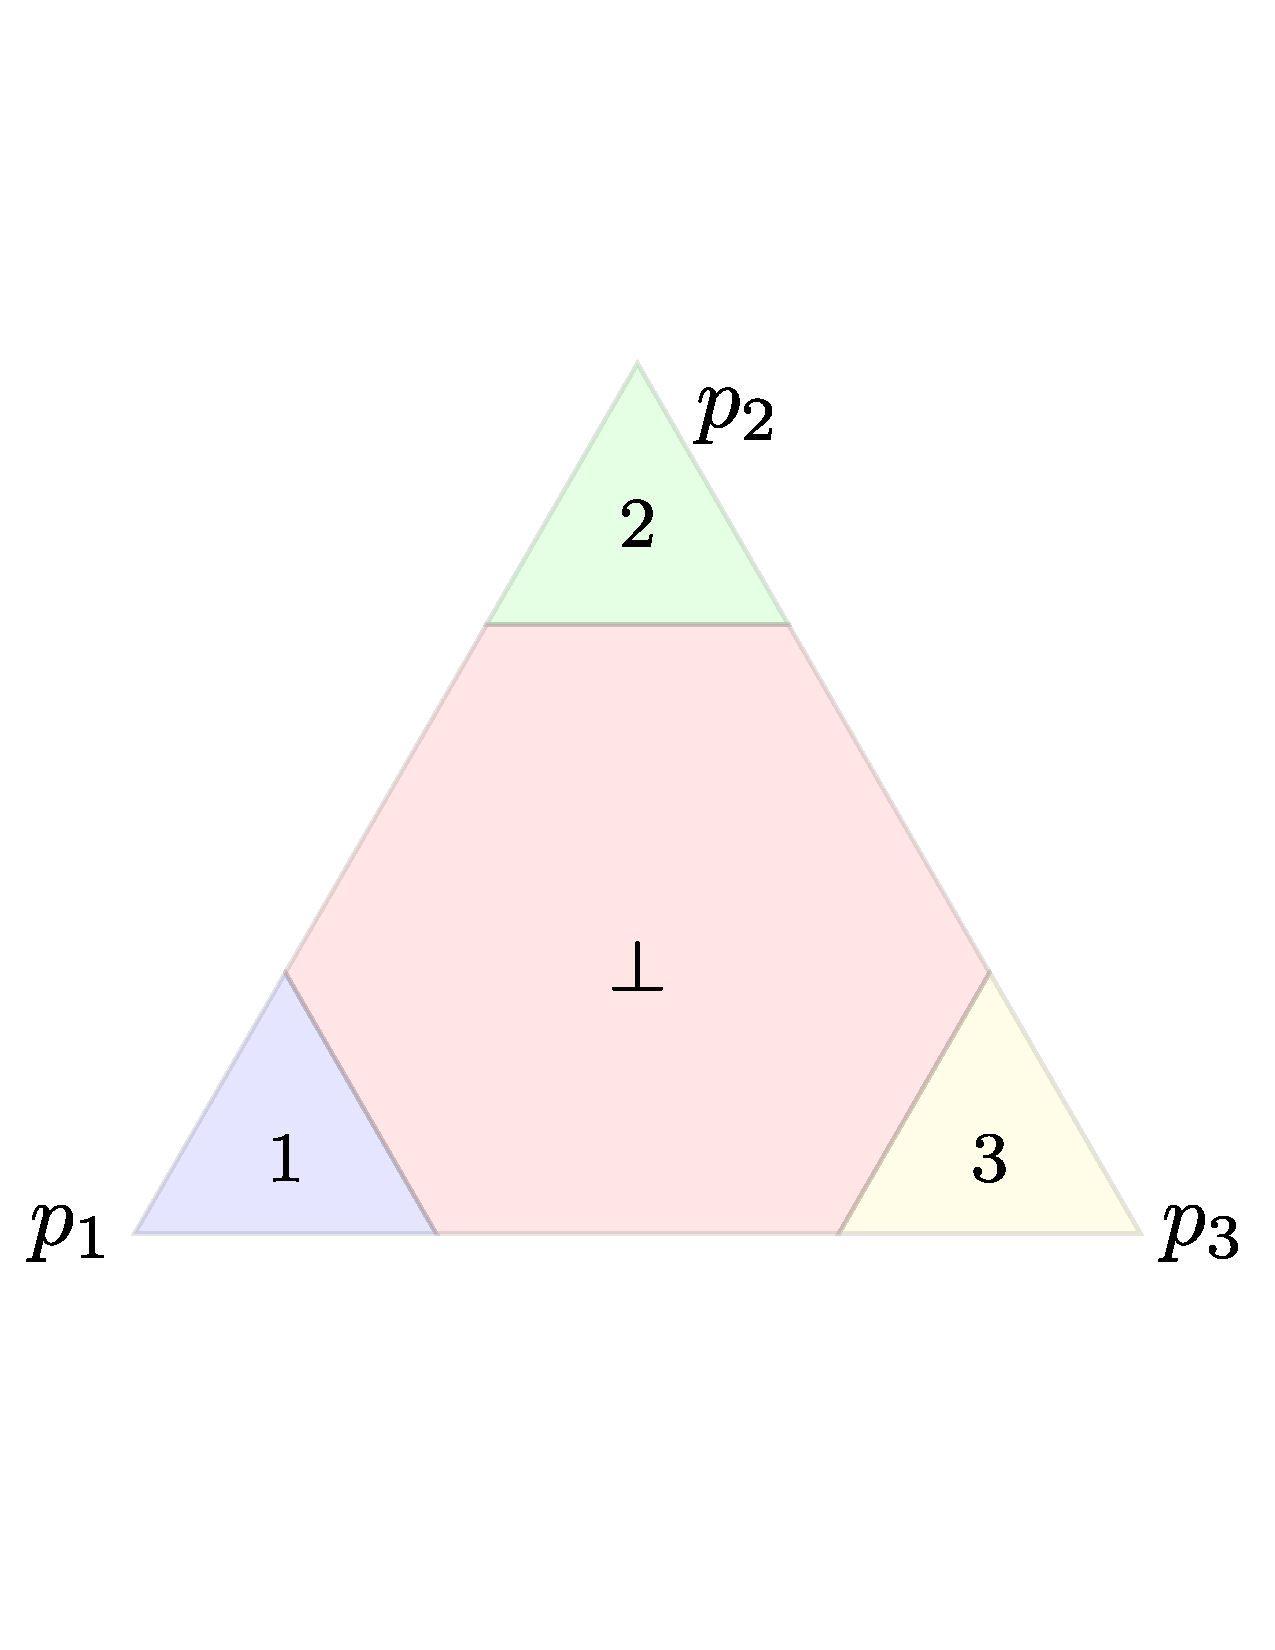
\includegraphics[width=\linewidth]{figs/abstain-alpha-point3.pdf}
	\end{minipage}%
\hfill
	\begin{minipage}{.32\textwidth}
	\centering
	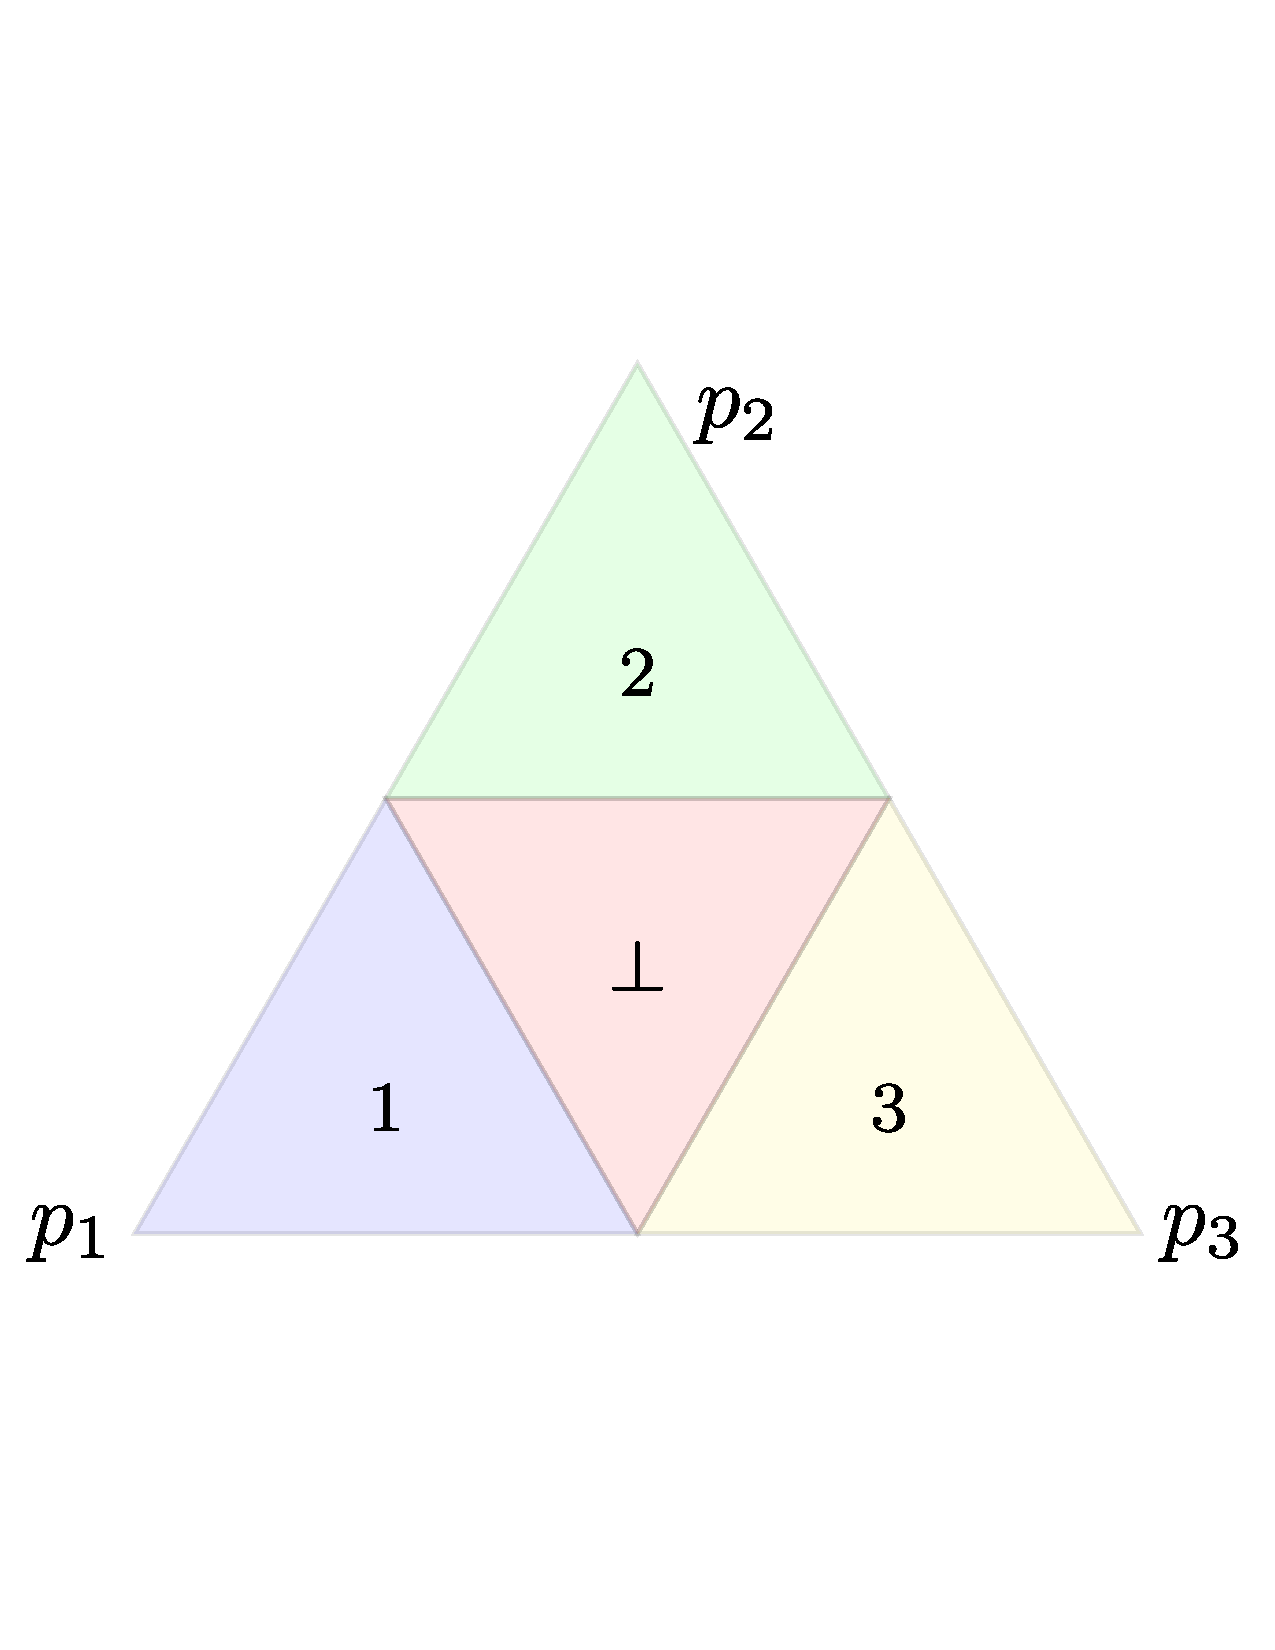
\includegraphics[width=\linewidth]{figs/abstain-alpha-half.pdf}
\end{minipage}%
\hfill
	\begin{minipage}{.32\textwidth}
	\centering
	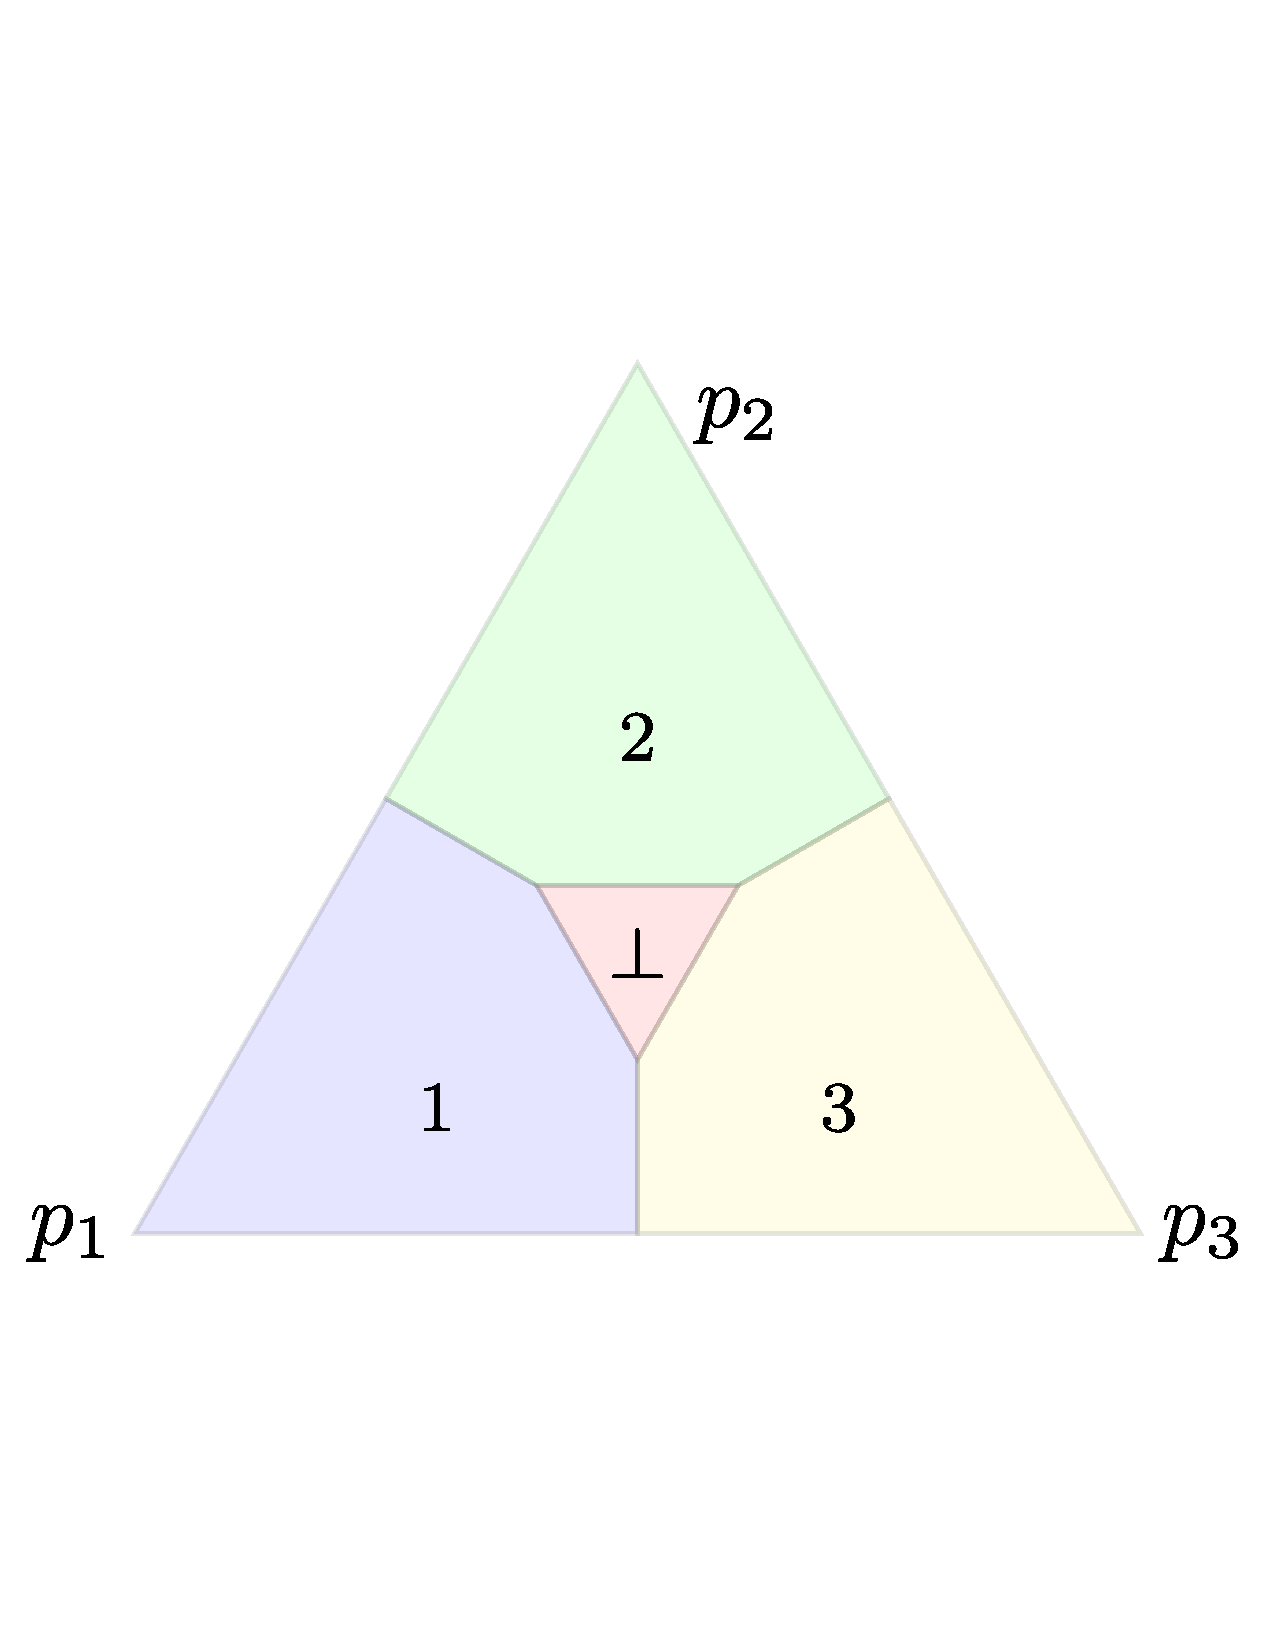
\includegraphics[width=\linewidth]{figs/abstain-alpha-point6.pdf}
\end{minipage}%
\caption{With $n = 3$, we can visualize values of $\gamma^\alpha(p)$ as one varies $p$ over $\simplex$.   Here, we vary $\alpha$ in each figure. $\alpha = 3/10$ (L), $\alpha = 1/2$ (M), $\alpha = 3/5$ (R).}
\end{figure*}

\section{Upper bounds on convex prediction dimension for the abstain loss}

\cite{ramaswamy2018consistent} introduces the Binary Encoded Prediction (BEP) surrogate or its natural extensions that is calibrated with respect to the abstain loss for $\alpha \in (0,1/2)$.
For this loss, we assign each outcome into a corner of the $\{-1, +1\}^d$ hypercube by a bijection $B : [n] \to \{-1+1\}^d$, where $d := \lceil \lg(n) \rceil$.

\begin{equation}
L^{BEP}(u,y) = \left( \max_{j \in [d]} B_j(y) u_j + 1 \right)_+ \tag*{BEP} 
\end{equation}


One of the primary strengths of this surrogate is the exponential reduction in the dimension $d$ of the surrogate report $u$, while still being calibrated over the entire simplex.
Previous surrogates such as One-vs-all~\citep{rifkin2004defense} and Crammer-Singer~\citep{crammer2001algorithmic} both require the dimension of $u$ to grow linearly, rather than logarithmically, with the number of outcomes.
Significant improvements to this dimensionality while the surrogate is consistent can lead to improvements in the efficiency of the optimization problem.
Moreover, the BEP surrogate is an embedding for $\ell^\alpha$, and therefore moves the optimal upper bound for both convex calibration and embedding to $\Theta(\lg(n))$.

\begin{theorem}
	$\embed(\ell^{\alpha}) \leq \lceil \lg(n) \rceil$ for values of $\alpha \in (0,1/2]$.
\end{theorem}
The upper bound is constructive and is true by the consistency of the BEP surrogate.
\begin{corollary}
	$\ccdim(\ell^{\alpha}) \leq \lceil \lg(n) \rceil$ for values of $\alpha \in (0,1/2]$.
\end{corollary}


\section{Lower bounds on consistent surrogates}

While abstain has a logarithmic upper bound on its convex calibration and embedding dimensions, to date there is a large gap between lower and upper bounds, especially as $n =: |\Y|$ grows.

\begin{openq}
	Construct a lower bound on $\ccdim(\ell^\alpha)$ for $\alpha \in (0,1/2)$.
\end{openq}

\begin{openq}
	Construct a lower bound on $\ccdim(\ell^\alpha)$ for $\alpha \in (1/2, (n-1) / n)$.
\end{openq}

We conjecture the bound is tight, though, unlike upper bounds, lower bounds on convex calibration dimension are not constructive.

\begin{conjecture}
	For $\alpha = 1/2$, the bound $\ccdim(\ell^\alpha) = \lceil \lg(n) \rceil$ is tight.
\end{conjecture}

\begin{conjecture}
	For $\alpha < 1/2$ and $n \geq 4$, we have $\ccdim(\ell^\alpha) < \lceil \lg(n) \rceil$. \jessiet{Is this true?  IIRC, we though it might be $\log_{1/\alpha}$ at one point.}
\end{conjecture}

Since embedding is a special case of convex calibration dimension, we also pose open questions on the embedding dimension; it is currently an open problem to understand if these two are equal.
%\begin{proposition}
%	The BEP surrogate \jessie{or an $\alpha$-appropriate variation} embeds $\ell^\alpha$ for $\alpha \in (0,1/2]$.
%\end{proposition}


\begin{proposition}
	$\ccdim(\ell^\alpha) \leq \embed(\ell^\alpha)$.
\end{proposition}
\begin{proof}
	If $L$ embeds $\ell$, then it is calibrated with respect to $\ell$ by~\citep[Theorem 3]{finocchiaro2019embedding}.
\end{proof}


\begin{openq}
	Construct a lower bound on $\embed(\ell^\alpha)$ for $\alpha \in (0,1/2)$.
\end{openq}

\subsection{Baby steps} \jessie{move these up to serve as intuition for the conjectures?}
\begin{theorem}[\citep{finocchiaro2020embedding} Proposition 1]
	For $\alpha \leq 1/2$ with $n = 3$, we observe $\embed(\ell^\alpha) = 2$.
\end{theorem}


\begin{theorem}[\citep{finocchiaro2020embedding}~Corollary 22]
	For $\alpha = 1/2$ with $n \geq 5$, we observe $\embed(\ell^\alpha) \geq 3$.
\end{theorem}

%\begin{openq}
%	Is $\ccdim(\ell^{1/2}) = \Theta(\lg(n))$?
%\end{openq}
%
%\begin{openq}
%	Given $\alpha \in (0,1/2]$, and $n$, what is $\ccdim(\ell^{\alpha})$?
%\end{openq}

\section{Future work and Conclusions}
\jessie{Note that actually strictly more efficient than learning the mode}
While upper bounds on the convex calibration dimension of the abstain loss exist, they are far from tight.
For $\alpha \leq 1/2$ and $n \geq 3$, the bounds we know simply state $2 \leq \ccdim(\ell^\alpha) \leq \embed(\ell^\alpha) \leq \lceil \lg(n) \rceil$.
As $n$ grows large, as in extreme classification, the gap provided by this bound is very large.

The next conjecture suggests that embedding is a sufficient framework to study convex calibration dimension.
\begin{openq}
	For any $\alpha \in (0,1/2]$, is $\ccdim(\ell^\alpha) = \embed(\ell^\alpha)$?
\end{openq}

If true, this would suggest that we can use tools from embedding techniques to characterize the convex calibration dimension.
Some of these tools include the use of Minkowski sums to calculate the subgradient sets of the expected loss of embedded reports at various distributions and a quadratic feasibility program whose solution yields subgradient sets at embedded points for a convex surrogate loss embedding the discrete loss.

However, it is not clear, if the lower bound on constructing a calibrated surrogate for the abstain loss is $\lceil \lg(n) \rceil$, why that is.
Current lower bounds come from the optimality condition that a report is in the property value at a distribution $p$ if and only if $\vec 0$ is in the subgradient set of the expected loss over $p$.
However, if tighter lower bounds come from monotonicity conditions concerned with the adjacency of level sets, we need new tools to study these bounds.


\newpage
\bibliographystyle{abbrvnat}
\bibliography{diss,extra}


\end{document}


% This document was modified from the file originally made available by
% Pat Langley and Andrea Danyluk for ICML-2K. This version was created
% by Iain Murray in 2018, and modified by Alexandre Bouchard in
% 2019 and 2020. Previous contributors include Dan Roy, Lise Getoor and Tobias
% Scheffer, which was slightly modified from the 2010 version by
% Thorsten Joachims & Johannes Fuernkranz, slightly modified from the
% 2009 version by Kiri Wagstaff and Sam Roweis's 2008 version, which is
% slightly modified from Prasad Tadepalli's 2007 version which is a
% lightly changed version of the previous year's version by Andrew
% Moore, which was in turn edited from those of Kristian Kersting and
% Codrina Lauth. Alex Smola contributed to the algorithmic style files.
